\section{Actividad No 08 – Enlaces} 
		
\begin{enumerate}[1.]
	\item El departamento de Recursos Humanos requiere un reporte que muestre las direcciones de todos los departamentos. Utilizar las tablas LOCATIONS y COUNTRIES. Mostrar el ID de la Ubicación (location\_id), dirección (street\_address), ciudad (city), estado o provincia (state\_province) y país (country\_name). % Utilizar NATURAL JOIN para producir el resultado.
	\begin{center}
	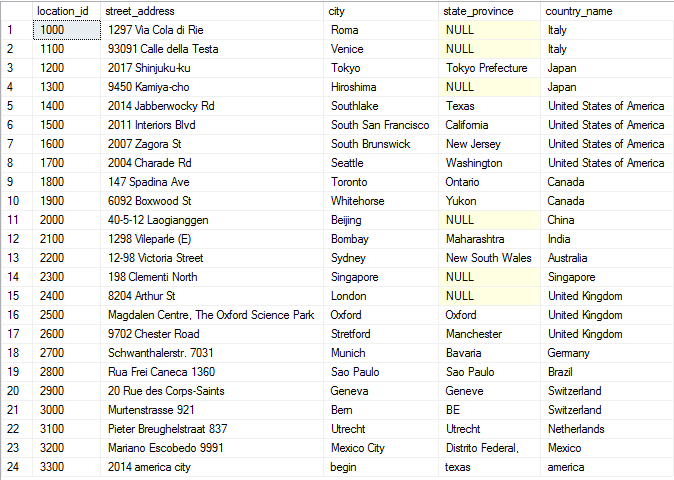
\includegraphics[width=5cm]{./Imagenes/actividad_08_01} 
	\end{center}


	\item El departamento de Recursos Humanos necesita un reporte de todos empleados, que muestres los apellidos de empleado (last\_name), el No de departamento (department\_id) y el nombre del departamento (depertment\_date) al cual pertenece. 

	\begin{center}
	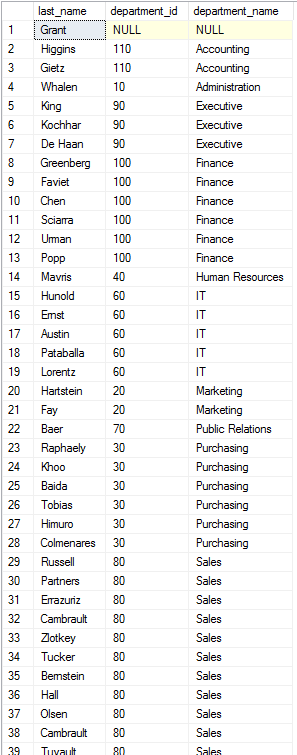
\includegraphics[width=5cm]{./Imagenes/actividad_08_02} 
	\end{center}

	\item El departamento de Recursos Humanos necesita un reporte de los empleados de la ciudad de Toronto. Mostrar los Apellidos, Puesto, No de Departamento y Nombre de Departamento de todos los empleados que trabajan en Toronto.

	\begin{center}
	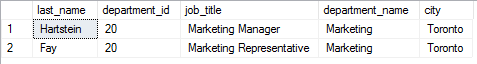
\includegraphics[width=5cm]{./Imagenes/actividad_08_03} 
	\end{center}

	\item Crear un reporte que muestre los Apellidos y No de Identificación de los empleados, asimismo también
debe mostrarse el Apellido y No de Identificaci\'on de su Administrador.

	\begin{center}
	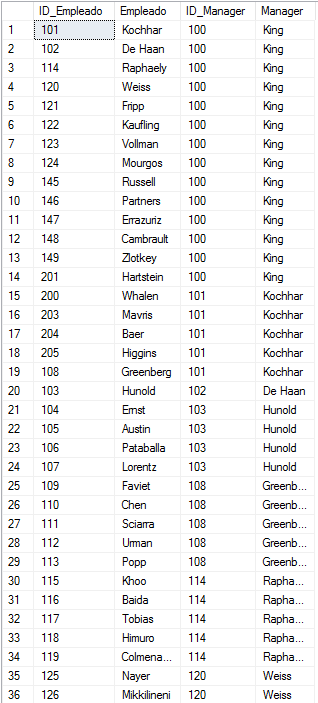
\includegraphics[width=5cm]{./Imagenes/actividad_08_04} 
	\end{center}

	\item Modificar la consulta anterior para que incluya tambi\'en a los empleados quienes no tienen Administrador asignado.

	\begin{center}
	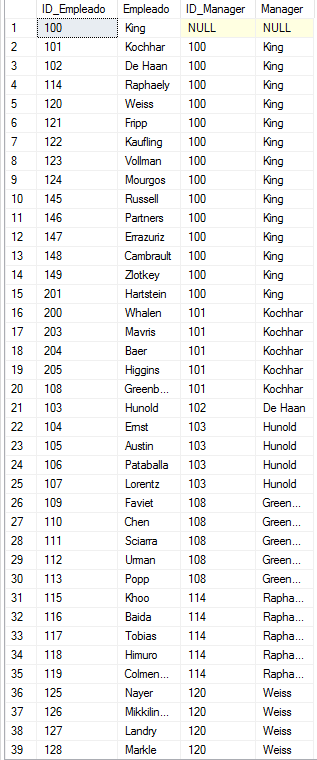
\includegraphics[width=5cm]{./Imagenes/actividad_08_05} 
	\end{center}

	\item Crear un reporte que muestre los No de Departamento y Apellidos de todos los empleados, asimismo adicionar una columna con los Apellidos de todos empleados que trabajan en el mismo departamento. Etiquetar esta columna como Colega.
	\item El departamento de Recursos Humanos requiere un reporte de todo el personal que fue contratado después del empleado apellidado ‘Davies’. Crear un reporte que muestre el apellidos y fecha de contrataci\'on de todo los empleados contratado después de ‘Davies’.
	\item El departamento de Recursos Humanos requiere de un reporte que el apellido del empleado, fecha de contrataci\'on del empleado, apellido del administrador, fecha de contratación del administrador. Para todos aquellos empleados que fueron contratados antes que sus Administradores.
\end{enumerate}

